\documentclass{article}
\usepackage[left=2.7cm, right=2.7cm, top=3cm]{geometry} % Change margins
\usepackage{mathtools} % falign
\usepackage{amsmath} % Basic maths
\usepackage{amssymb} % For some symbols
\usepackage{bm} % bold math
\usepackage{tikz} % For drawing trees
\usepackage{tikz-qtree} % For drawing trees
\usetikzlibrary{trees, positioning, arrows.meta, calc} % For drawing trees
\usepackage{xcolor} % Colouring equations
\usepackage{fancyhdr} % Cool headers
\usepackage{tabularx} % Fixed tables
\usepackage{graphicx}
\usepackage{multirow} % table merge row
\usepackage{color, colortbl} % colouring
\usepackage{tcolorbox} % for boxed stuffs, text + math mode
\usepackage{alltt} % better verbatim
\usepackage{wrapfig} % wrapping images with env wrapfigure
\usepackage[hidelinks]{hyperref}
\usepackage{booktabs} % better tables
\usepackage{float} % float tables
\usepackage[underline=false]{pgf-umlsd} % uml sequence diagrams
\restylefloat{table}
\usepackage{minted} % code highlighting
\usepackage{longtable} % tables that span multiple pages
\usepackage{enumitem} % \begin{enumerate}[label=(\alph*)]
\usepackage{pgfplots}
\usepackage{xifthen}% provides \isempty test
\usepackage[font=small,labelfont=bf]{caption}

\usepackage{subfig}

\def\BibTeX{{\rm B\kern-.05em{\sc i\kern-.025em b}\kern-.08em
    T\kern-.1667em\lower.7ex\hbox{E}\kern-.125emX}}

\pgfplotsset{compat=1.16} % Backwards compatibility

\usepackage{xargs} % Use more than one optional parameter in a new commands

\usepackage[sorting=none]{biblatex}
\addbibresource{refs.bib}

% A really nice TODO package and helpers
% https://tex.stackexchange.com/questions/9796/how-to-add-todo-notes
\setlength {\marginparwidth }{2cm}
\usepackage[colorinlistoftodos,prependcaption,textsize=tiny]{todonotes}
\newcommandx{\todoany}[2][1=]{\todo[inline,#1]{[\sectionlabel{}]~#2}}
\newcommandx{\todojim}[2][1=]{\todo[linecolor=red,backgroundcolor=red!25,bordercolor=red,inline,#1]{[\sectionlabel{}]~\textbf{Jim}:~#2}}
\newcommandx{\tododuke}[2][1=]{\todo[linecolor=blue,backgroundcolor=blue!25,bordercolor=blue,inline,#1]{[\sectionlabel{}]~\textbf{Duke}:~#2}}
\newcommandx{\tododhruv}[2][1=]{\todo[linecolor=green,backgroundcolor=green!25,bordercolor=green,inline,#1]{[\sectionlabel{}]~\textbf{Dhruv}:~#2}}

\hypersetup{
  colorlinks=true,
  urlcolor=blue,
  linkcolor=black,
  citecolor=black
}

% circled numbers
\newcommand*\circled[1]{\tikz[baseline = (char.base)]{%
            \node[shape=circle,draw,inner sep=2pt] (char) {#1};}}%

% For use in align*
\newcommand*\mathcomment[1]{&&{#1}}
\newcommand*\mathcommentt[1]{&&{\text{#1}}}

\usepackage{amsthm} % For Proofs
\newtheorem*{remark}{Remark}
\renewcommand\qedsymbol{}

\begin{document}

\pagestyle{fancy}
\fancyhf{}
\lhead{COMP9491: Project Report}
\rhead{Duck News Reporters}
\cfoot[C]{\thepage}

\renewcommand{\headrulewidth}{1pt}
\renewcommand{\footrulewidth}{0.5pt}

\newcommand{\sectiontitle}{}
\newcommand{\subsectiontitle}{}
\newcommand{\sectionlabel}{\ifdefempty{\subsectiontitle}{\sectiontitle}{\sectiontitle/\subsectiontitle}}
\newcommand{\newsection}[1]{\section{#1}\renewcommand{\sectiontitle}{#1}\renewcommand{\subsectiontitle}{}}
\newcommand{\newsubsection}[1]{\subsection{#1}\renewcommand{\subsectiontitle}{#1}}

% \begin{noindent}
\newcommand{\articlecontent}[1]{%
	\ifthenelse{\equal{#1}{118real}}{FBI Director James Comey said Sunday that
	the bureau won't change the conclusion it made in July after it examined
	newly revealed emails related to the Hillary Clinton probe.

	``Based on our review, we have not changed our conclusions that we
	expressed in July with respect to Secretary Clinton'' Comey wrote in a
	letter to 16 members of Congress. [...]
	}{}%
  \ifthenelse{\equal{#1}{128real}}{[...]I have a prediction. I know exactly what
  November 9 will bring. Another day of God’s perfect sovereignty.

  He will still be in charge. His throne will still be occupied. He will still
  manage the affairs of the world. Never before has His providence depended on a
  king, president, or ruler. And it won’t on November 9, 2016. “The LORD can
  control a king’s mind as he controls a river; he can direct it as he pleases”
  (Proverbs 21:1 NCV).
  
  On one occasion the Lord turned the heart of the King of Assyria so that he
	aided them in the construction of the Temple.  On another occasion, he stirred
	the heart of Cyrus to release the Jews to return to Jerusalem. [...]}{}%
  \ifthenelse{\equal{#1}{2fake}}{Washington, D.C. – South African Billionaire,
  Femi Adenugame, has released a statement offering to help African-Americans
  leave the United States if Donald Trump is elected president. According to
  reports, he is offering \$1 Million, a home and car to every Black family who
  wants to come to South Africa.

  Concerns about Donald Trump becoming president has prompted a South African
  billionaire to invest his fortune in helping African-Americans leave the
  United States to avoid further discrimination and inequality. [...]}{}%
  \ifthenelse{\equal{#1}{10fake}}{The Internet is buzzing today after white
  supremacist presidential candidate Donald Trump was caught by hotel staff
  snorting cocaine.

  Maria Gonzalez an employee at the Folks INN \& Suites Hotel in Phoenix brought
  room service to his room witnessed it all.
  
  ``When I walked in I saw 3 naked prostitutes and maybe 100,000 in hundred
  dollars bills and a mountain of white powder on the table, I thought it was a
  dog on the floor sleep but it was his hair piece, he was bald and sweating
  like crazy.'' [...]}{}%
	\ifthenelse{\equal{#1}{15fake}}{After hearing about 200 Marines left
	stranded after returning home from Operation Desert Storm back in 1991,
	Donald J.Trump came to the aid of those Marines by sending one of his planes
	to Camp Lejuene, North Carolina to transport them back home to their
	families in Miami, Florida.

	Corporal Ryan Stickney was amongst the group that was stuck in North
	Carolina and could not make their way back to their homes. [...]
	}{}%
  \ifthenelse{\equal{#1}{34fake}}{It has been more than fifteen years since Rage
  Against The Machine have released new music. The members of the band have
  involved themselves in various other projects during their lengthy hiatus, but
  one pressing issue has forced the band to team up once again.

  In a statement posted online, Rage Against The Machine announced they would be
	releasing a brand new album aimed at spreading awareness about ``how awful
	Donald Trump is''. [...]
	}{}%
}
% \end{noindent}

\title{\textbf{Duck News Reporters: Automated fake news detection through contextual similarity comparison}\\\vspace*{12pt}\large{COMP9491: Applied Artificial Intelligence --- Project Report}}
\author{%
  Dhruv Agrawal\\
  \texttt{z5361800@unsw.edu.au}
  \and
  Duke Nguyen\\
  \texttt{z5398432@unsw.edu.au}
  \and
  Jim Tang\\
  \texttt{z5208565@unsw.edu.au}
}

\maketitle
\thispagestyle{empty}

\listoftodos % DELETE THIS BEFORE SUBMIT

\newsection{Introduction}

\todoany{Describe the problem domain and aim of study, briefly introduce the developed methods and summarise your experimental findings}

\newsection{Related work}

\tododhruv{Describe the current state-of-the-art or related literature in this problem domain}

\newsection{Methods}

\begin{minipage}{\textwidth}
  \begin{wrapfigure}{r}{0.65\textwidth}
    \vspace*{-20pt}
    \centering
    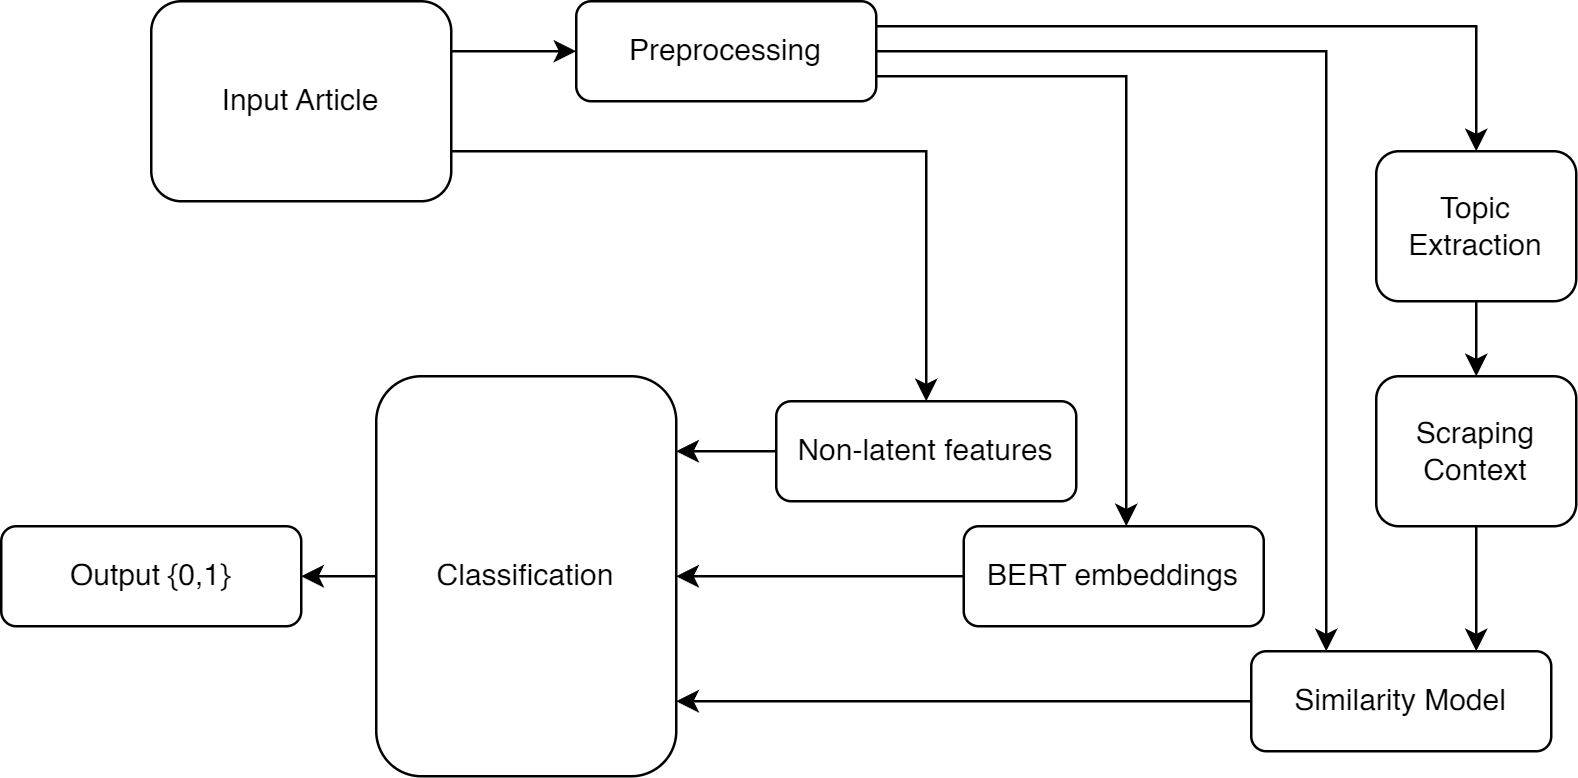
\includegraphics[width=0.6\textwidth]{img/pipeline.png}
    \caption{Our classification pipeline.}
    \label{pipeline}
  \end{wrapfigure}

  Figure~\ref{pipeline} shows our mostly linear classification pipeline. After preprocessing and tokenization, we extract contextual articles which are fed into a similarity model to form our first feature. Additionally, non-latent features from raw text and BERT embeddings form the rest of our features. The concatenation of all the features are fed into our classification models which infers a binary classification label.
\end{minipage}

\newsubsection{Preprocessing and tokenization}

Before extracting any features, we will preprocess our input and convert the long form text into tokens. We perform the following preprocessing methods in order:

\begin{quote}
  \textbf{Remove non-ascii:}\quad Our input articles contained unnecessary unicode tokens such as unicode double quotation marks. These can be removed safely since they do not add any extra semantics to the input articles and may confuse feature extraction.

  \textbf{Convert to lowercase:}\quad In our research, we converted all text to lowercase. However upon further analysis, converting all text to lowercase hid acronyms such as ``US'' which could have affected the main themes of the text. Further, all proper nouns such as names and places were also hidden. We will discuss this limitation in Section~\ref{limitation:preprocessing}.

  \textbf{Lemmatization:}\quad We used the \verb|nltk|~\cite{nltk} libaray to reduce words down to their lemma in the hopes of reducing the complexity within our text which may benefit feature extraction. This looks up the work in the WordNet corpus to get the lemma. Later in the research, we realised that this hypothesis may have not been accurate.

  Firstly the \verb|nltk| library we were using does not automatically detect the part of speech and will by default, only lemmatize nouns. While it is arguably better for us to maintain the tense of nouns, we are technically not lemmatizing fully. Secondly, from more research, lemmatization may not be ideal for BERT embeddings since it removes some semantics that could be learnt by the BERT model. We will discuss these limitations further in Section~\ref{limitation:preprocessing}.

  \textbf{Remove stopwords:}\quad Stopwords were removed from the text in order to reduce complexity.
\end{quote}

Apart from the above methods, we also tested removing punctuation. However, this was not used in the end since we added non-latent features to measure punctuation counts and also to maintain semantics for BERT.

After preprocessing, tokens are then generated based on any whitespace and punctuation in the remaining text. Table~\ref{preprocessing} shows samples of tokenized input articles.

\begin{table}
  \begin{center}
    \makebox[0pt]{\begin{minipage}{\paperwidth}
        \centering
        \subfloat{
          \begin{tabular}{cp{8cm}p{6cm}}
            \toprule
            ID & Article extract & Tokens\\
            \midrule
            118\_Real & \small{\articlecontent{118real}}
            & \small{['fbi', 'director', 'james', 'comey', 'said', 'sunday', 'bureau', 'change', 'conclusion', 'made', 'july', 'examined', 'newly', 'revealed', 'email', 'related', 'hillary', 'clinton', 'probe', '.', '"', 'based', 'review', ',', 'changed', 'conclusion', 'expressed', 'july', 'respect', 'secretary', 'clinton',\ldots]}\\
            \midrule
            15\_Fake & \small{\articlecontent{15fake}}
            & \small{['hearing', '200', 'marines', 'left', 'stranded', 'returning', 'home', 'operation', 'desert', 'storm', 'back', '1991', ',', 'donald', 'j', '.', 'trump', 'came', 'aid', 'marines', 'sending', 'one', 'plane', 'camp', 'lejuene', ',', 'north', 'carolina', 'transport', 'back', 'home', 'family', 'miami',\ldots]}\\
            \bottomrule
          \end{tabular}
        }
        \hfill
      \end{minipage}}
  \end{center}
  \caption{Examples of preprocessing and tokenization extraction on items in dataset.}
  \label{preprocessing}
\end{table}

\tododuke{Talk about doing average pooling of the entire output for future work instead of just using the CLS token}
% \tododuke{Cite: https://huggingface.co/docs/transformers/model_doc/bert, https://huggingface.co/bert-base-uncased}
\newsubsection{Feature --- BERT embeddings}
"BERT (Bidirectional Encoder Representations from Transformers) is a language representation model proposed by Devlin et al. It pretrains on unlabeled text using masked language modeling (MLM) and next sentence prediction (NSP). With a single output layer, BERT achieves state-of-the-art performance in various tasks. It outperforms other models in natural language processing, including GLUE score, MultiNLI accuracy, and SQuAD v1.1 and v2.0 Test F1. BERT uses absolute position embeddings, and inputs are usually padded on the right. The model masks tokens during training to predict the original sentence and distinguish consecutive or unrelated sentences." We will be using the implementation on HuggingFace with the 'bert-base-uncased'. We will extract the first 512 tokens of an article and pass it through bert-base-uncased, and retrieve the vector output of the CLS token as BERT features for our classification model.

\tododuke{Cite: Zhou \& Zafarani, Garg \% Sharma, Hornn \& Adali}
\newsubsection{Feature --- Non-latent features} \label{section:non-latent-feat}
From our literature review and survey, we are able to identify a significant amount of non-latent features. After combining features that are similar, and removing features which we cannot calculate due to the need for proprietary softwares (i.e. LIWC), or due to the computational complexity of the algorithms, or related reasons, we are able to identify 81 numerical features suitable for our experiments. After synthesising their categorisations in the original articles, we come up with a grouping of 7 main categories (with their abbreviation in brackets), with each feature being able to calculated with a few methods:
\begin{itemize}
    \item Diversity (div): number of unique words, or percentage of all unique words of a particular part of speech (e.g. noun, verb)
    \item Quantity (quant): number of words, or percentage of all words of a particular part of speech or linguistic unit (e.g. noun, adjective, quote)
    \item Sentiment (senti): number of linguistic features denoting sentiment (e.g. exclamation mark, all-cap words), or sentiment measurement (polarity, subjectivity)
    \item Pronoun (pron): number of pronouns of a specific class (e.g. first person singular pronoun: I, me, my, mine)
    \item Average (avg): average number of linguistic unit \texttt{a} per linguistic unit \texttt{b} (e.g. characters per word)
    \item (Median) Syntax Tree Depth (med\_st): the median syntax tree depth of a given unit (e.g. median noun phrase syntax tree depth)
    \item Readability (read): different readability indices (e.g. gunning-fog, coleman-liau)
\end{itemize}

\tododuke{MAYBE I COULD PUT THE EXCEL TABLE IN THE APPENDIX OF ALL FEATURES}

% https://github.com/dukeraphaelng/ducknewsreporter/blob/main/src/non_latent_features.py
The feature names are designated using the format "\texttt{category}\_\texttt{featureType}\_\texttt{calculationMethod}", where category is the abbreviated \texttt{category}, \texttt{featureType} is the feature type within the category, (due to page limitation, a complete table would not be provided here, but they are available in the docstring description for each category method here: [CITATION HERE]), and \texttt{calculationMethod} is \texttt{sum} when it is the count (i.e. number of) the respective feature, or the default method; it is \texttt{percent} when it is a percentage of all words or unique word in diversity, quantity, or pronoun. Figure \ref{box-plot} is a box plot of all the non-latent features by their scale of power of 10. The majority of features are between the range of $[10^{-2}, 10^{1}]$. Several quantity and some diversity features are in the higher range of $[10^2, 10^3]$. 

\begin{figure}[H]
  \centering
  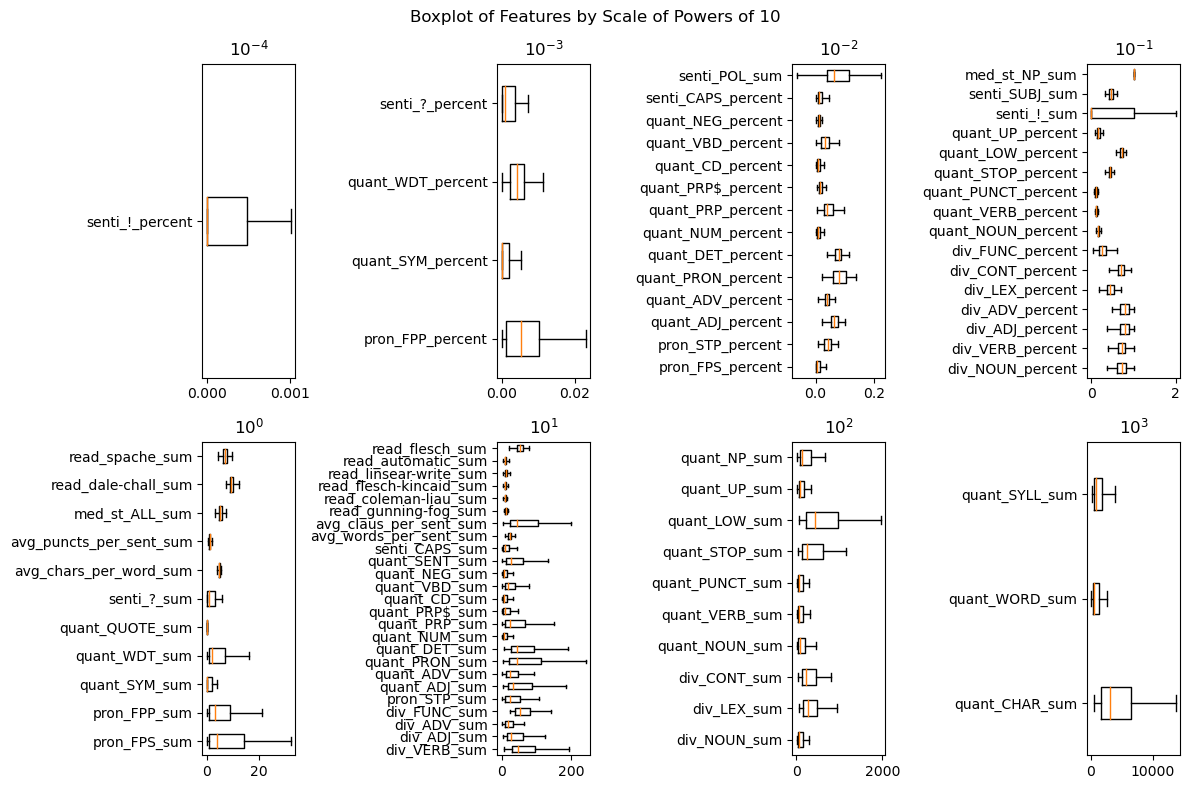
\includegraphics[width=\textwidth]{img/non_latent_box_plot.png}
  \caption{Non Latent Box Plot Features}
  \label{box-plot}
\end{figure}

We can then apply ANOVA on these non-latent features against the labels, and filter for those with a p-value less than the $\alpha$ significance level of 0.05. We identify that the removed features account to almost half of all features, and they include readability indices, the syntax tree depth features, and a few features from other categories, and diversity features are all below $\alpha$. We then apply Pearson correlation amongst the selected features and identify all correlation clusters. The matrix is available in Appendix \ref{appendix:correlation-matrx}. Afterwards, we can apply a selection method on the cluster where we remove all but one with the lowest p-value, specifically, we sort the selected features by p-value in ascending order with the lowest p at the front of the list, we then search for all features which have a correlation of at least $0.95$ and remove them from the current list, and continue until the end. Figure \ref{fig:non-latent-feat-prune} shows our results. After grouping them by their original category, we have the following counts, totalling to 29 features, which we will use for our classification models:
\begin{itemize}
    \item Diversity: 9 features
    \item Quantity: 12 features
    \item Pronoun: 2 features
    \item Sentiment: 3 features
    \item Average: 1 feature    
\end{itemize}

\begin{figure}[H]
  \centering
  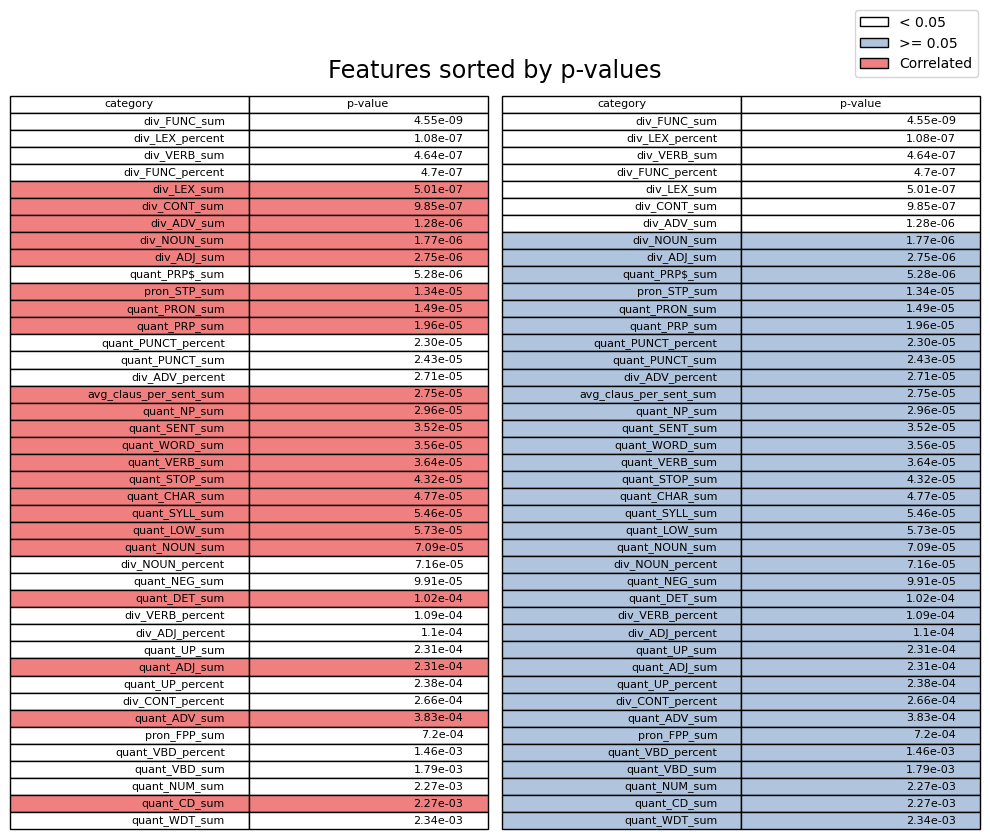
\includegraphics[width=\textwidth]{img/non_latent_feat_prune.png}
  \caption{Non-Latent Feature Pruning}
  \label{fig:non-latent-feat-prune}
\end{figure}

\newsubsection{Feature --- Similarity model}

\tododuke{I changed subsubsection* to subsubsection to label and reference them here}
\tododuke{I think the order should be BERT -> non latent -> Similarity as this makes more sense}
\tododuke{Explain the point of similarity model: Hypothesis - we hypothesize that articles that are real vs false are more dissimilar than articles that are both real. We assume context articles are real}
\tododuke{i havent pulled in the latest changes yet, so Im not sure what Dhruv has written, but atm the report in the similarity section doesnt explain why we are doing this, whats our hypothesis, what we are doing to confirm it, and so on. ie we are expecting that the similarity metric makes a difference }
The similarity model consists of two main components: scraping context articles for input article, and outputting a similarity metric for the pair. The first step involves \textbf{summary extraction} (Section \ref{section:summary-extraction}) of input articles into keywords, and perform \textbf{article scraping} (Section \ref{section:article-scraping}) using the associated keywords for context articles. The second step involves \textbf{article vectorisation} (Section \ref{section:article-vectorisation}) of the input-context article pair, and feeding them into different \textbf{similarity metrics} (Section \ref{section:similarity-metric}), choosing for one differentiates the Real and Fake distributions the most distinctly.

\tododuke{Not sure what to do with the commented-out paragraph below after adding above intro/summary}
% One of the core aspects of our research was the ability to automatically gather articles that give some context to each input article. Our approach summarizes the input article so it can be used to find contextual articles. These articles can then be used for comparison to the input article.

\subsubsection{Summary extraction} \label{section:summary-extraction}

To get the context articles, we need to summarize the main topic of our input article down to at most 10 keywords. We use the Python \verb|gensim|~\cite{py-gensim} library which provides various topic modelling interfaces for text inputs. We use the \verb|ldamodel| which implements Latent Dirichlet Allocation (LDA) to extract a single topic. LDA is a probabilistic model where the idea is you have a number of documents representing some latent topics characterized by a distribution over words. By feeding in the preprocessed sentences of our input article, we are able to get the main themes. We sort the output keywords by the probability they represent the topic then cap the amount of words to 10 at most.

For the scope of our research, we are able to perform manual validation of the summaries extracted to check the summary represented the article content well. Table~\ref{summary-extraction} shows some samples of items in our dataset after applying LDA. We see that while the summaries extracted are not perfect, they still represent the general meaning of the article. Two common issues we saw were:
\begin{itemize}
  \item Unordered words in the summary --- words representing the topics seemed to be unordered. To a human reading the summary by itself, they might be able to see that the words are all keywords of the article but put together in a sentence, will not completely make sense. We hypothesize that this could have caused sub-optimal results when we started scraping articles using the summaries.
  \item Appearance of stop words and other meaningless non-topic words in the summary --- As a flow on issue from our preprocessing, our summary was left with words such as ``wa'' (from ``was'') or ``ha'' (from ``has''). This would have impacted the meaning of our summary and later article scraping.\label{summary-extraction:bad-words}
\end{itemize}
We will discuss the possibility of extracting better summaries using a more robust model in Section~\ref{limitation:summary-extraction}.

\begin{table}
  \centering
  \begin{tabular}{cp{8cm}p{3cm}}
    \toprule
    ID & Article extract & Summary\\
    \midrule
    118\_Real & \small{\articlecontent{118real}}
    & email review fbi clinton said july comey news new wa\\
    \midrule
    15\_Fake & \small{\articlecontent{15fake}}
    & home marines trump wa stickney way north plane family\\
    \bottomrule
  \end{tabular}
  \caption{Examples of summary extraction on items in dataset.}
  \label{summary-extraction}
\end{table}

\subsubsection{Article scraping} \label{section:article-scraping}

We feed the summary of the input article into Google News and collect the top three articles. We use Google News since it essentially provides a free PageRank algorithm which we can leverage to get the most popular articles during the time period. We will treat the articles we find as Real articles for purposes of comparison, i.e.\ an input article that is very different to our contextual article is likely to be Fake.

For our research, we will only manually feed in all summaries for our dataset. Our motivation for this research was to develop a tool that a user could potentially use to figure out if the current news they are reading contains misinformation. We acknowledge there exists APIs that provide either a wrapper around Google News or implement their own news search algorithm that we could have looked into. However, given the size of the dataset and our scope, this was not necessary to demonstrate our system.

\begin{quote}
  \textbf{SETUP:} We use a virtual machine with a freshly installed latest version of Google Chrome. Searches are condicted in ``Incognito Mode'' tabs. We also use a VPN to the West coast of the US. These invariants serve the main purpose so that Google's does not give any personalized results based on a browser fingerprint or IP address. We chose the US as the VPN destination since our dataset articles were extracted from US news sources and we wanted to scrape for articles with a similar style of writing. If you were to use the tool in Australia, Google would usually return articles from local sources. We restrict our scope to specifically this dataset rather than train on a wide dataset from all sources.

  Another invariant we implement is to add a \verb|before:2020| to our summary. This forces Google News to only find articles before this year so that the news we get won't be from recent news. A common discussion topic from our dataset was Donald Trump's 2016 election campaign and we know that the news regarding Trump in 2023 is much different to that of 2016. This makes sense as we are not using a very recent dataset so clamping the date we find contextual articles assumes that if were looking for fake articles at the time of reading the imput article, we wouldn't have too much future articles available.

  \textbf{PROCESS:} We attempt to get the top three articles and save the URL for each input article. Not all summaries returned three articles so we perform scraping in three passes:
  \begin{enumerate}
    \item We enter the whole summary without any changes. This is the most ideal approach and most machine-replicable. This covered 70\% of our dataset.
    \item Still performing only generic actions, we remove any~\hyperref[summary-extraction:bad-words]{\color{blue}bad words} or non-important connectives then searched again. This should still be machine-replicable with further work. This covered the next 20\% of our dataset.
    \item For the last 10\% of our dataset, we had to manually look at the input article content and summary generated to figure out why we still received no results. Our hypothesis was that this was a combination of our non-tuned summary extraction and the fact that some \emph{outrageous} Fake articles simply didn't have any similar articles that could be found. We will discuss this limitation in Section~\ref{limitation:article-scraping}.
  \end{enumerate}
  From the above passes, we were not able to find context articles for four input articles described in a table in Appendix~\ref{appendix:article-scraping}. Furthermore, we were only able to find one or two articles for some inputs but we can still continue with our similarity model.
\end{quote}

\begin{figure}[H]
  \centering
  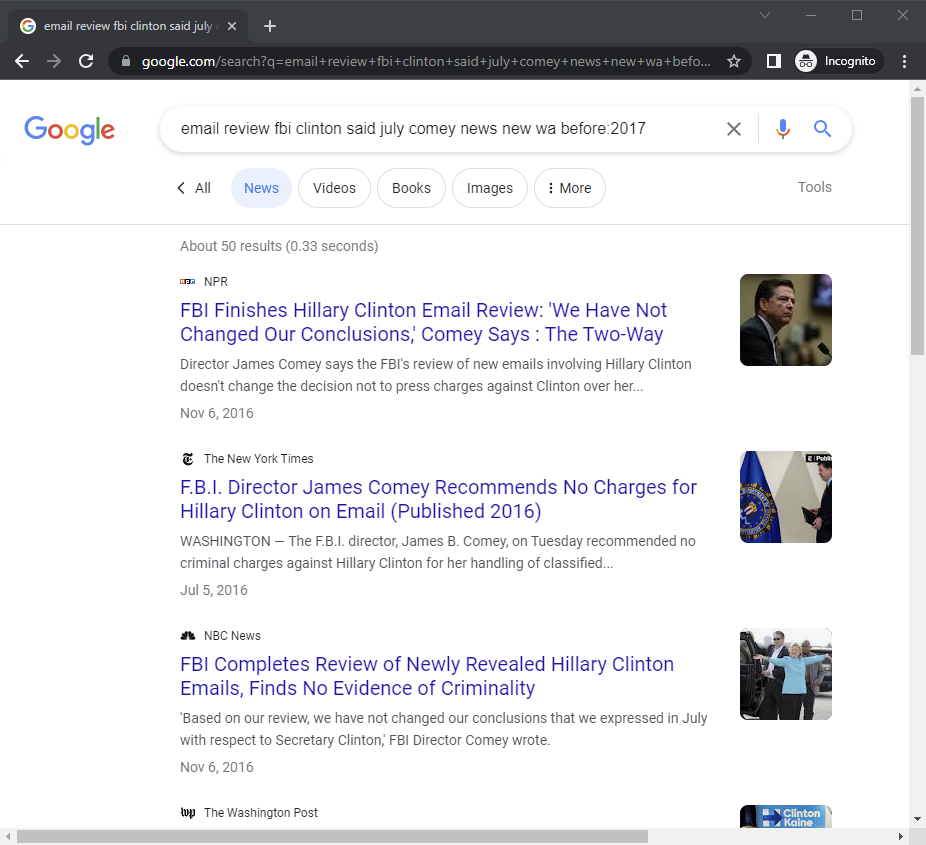
\includegraphics[width=0.4\textwidth]{img/chrome-article-scraping.png}
  \caption{Sample of articles found in Google after searching an article summary.}
\end{figure}

\noindent
After gathering three URL links for each context article, we use the Python \verb|newspaper3k|~\cite{py-newspaper} library to download the article and automatically extract its title and content.

% \subsubsection*{Similarity model}
% Once we have context articles for each input article, we can apply a transformation on the two to obtain their vector representations (a process called article vectorisation), after which we can apply a metric on the two article vectors and output a numeric value representing the similarity between the two corresponding articles (a process which we call similarity metric calculation). We will now discuss different approaches to article vectorisation and similarity metric calculation.

\subsubsection{Article vectorisation} \label{section:article-vectorisation}
\tododuke{Cite one more article here that also does the same similarity metric calculation}
\tododuke{Future work: vectorise the title and not just the body}
\tododuke{Future work: detect similarity between body and title pair}
Alsuliman, et. al propose two different ways to vectorise the articles: TF-IDF, word2vec \cite{alsuliman2022social}. In addition to these two vectorisation methods, we propose a third - 'non-latent vectoriser'. Vectorisation methods will now be inspected in close details.

% https://scikit-learn.org/stable/modules/generated/sklearn.feature_extraction.text.TfidfTransformer.html#:~:text=The%20formula%20that%20is%20used,document%20frequency%20of%20t%3B%20the
\textbf{TF-IDF}, which stands for term frequency times inverse document frequency, is a 'common term weighting scheme in information retrieval' \cite{scikit-learn}. The formula given as follows:

\[\frac{article.count(term)}{len(article)} * log_2(\frac{len(articles)}{df(articles, term)} + 1)\]

The first term is the term frequency, and the second term is the inverse document frequency, where \texttt{article} is the article we are applying TF-IDF on, \texttt{article.count(term)} is the frequency of \texttt{term} in \texttt{article}, \texttt{len(article)} is the number of words in the article, \texttt{len(articles)} is the number of articles, \texttt{df(articles, term)} is the document frequency of \texttt{term} in our \texttt{articles} dataset, or the number of articles that contains this term  \cite{scikit-learn}. The formula given has a '+1' term in idf so that the algorithm would not ignore terms that appear in all articles, this is the \texttt{sklearn} implementation and differs from the standard textbook formula which has the '+1' in the denominator in log2 of idf  \cite{scikit-learn}. TF-IDF will be fitted on the original dataset of input articles (for \texttt{articles} in IDF term), then be used as vectorize to transform both the input and context articles. We will apply TF-IDF in two n-gram ranges of (1,1) and (1,2).

\tododuke{ChatGPT}
\tododuke{Cite: https://radimrehurek.com/gensim/models/word2vec.html}
\tododuke{Cite: https://code.google.com/archive/p/word2vec/}
\tododuke{Cite Alsuliman or the article that pioneered the use of document vec as the average vec in this case}
\textbf{Word2Vec}, "a popular word embedding technique, represents words in a vector space to capture semantic similarities. Introduced by researchers at Google in 2013, it uses CBOW and Skip-gram architectures to learn embeddings from large text corpora. CBOW predicts target words from context, while Skip-gram predicts context from targets. The model optimizes to make similar words closer in vector space (ChatGPT)". We will be using the gensim implementation of word2vec using the pretrained 'word2vec-google-news-300' model which is trained on the Google News dataset of about 100 billion words containing 3 million words and phrases in 300 dimensions. We chose this model due to the similarity between the domain of its dataset and out dataset being news. To calculate the article vector, we retrieve the vector of every single word in an article, existing those that do not exist in the embeddings, and then taking the average from the list. The calculation of the article vector follows the work of Alsuliman et al.

\textbf{Non-Latent Vectorizer}
The non-latent vectorizer uses the non-latent feature selected in Section \ref{section:non-latent-feat} and apply them on an article into a vector. This is the non-latent vector presentation of the respective article.

\subsubsection{Similarity metric calculation} \label{section:similarity-metric}
\tododuke{Future work: learn a model instead of using metrics.}

Alsuliman et al. proposes three different metrics to calculate the similarity between two documents: cosine distance, word appearance (word app), matching score \cite{alsuliman2022social}. In addition, we also propose a third metric being the harmonic mean of the three, to harmonise any statistical difference and incorporate all distributional differences between the measures. The formula for each metric will now be discussed:

\tododuke{CosineDist: cite: https://docs.scipy.org/doc/scipy/reference/generated/scipy.spatial.distance.cosine.html}
\tododuke{CosineDist: cite: https://scikit-learn.org/stable/modules/metrics.html}

\noindent \textbf{Cosine distance} is calculated as one minus the cosine similarity of two vectors $u$ and $v$. The cosine similarity is the cosine of the angle between the two vectors (calculated as the dot product of $u$ and $v$) divided by the product of the Euclidean L2 norm of the two vectors to scale the range to [0, 1]. Lower values denote higher similarity between the two vectors, and vice versa. The formula is given as follows:
\[ 1 - \frac{u \cdot v}{\lVert u \rVert \lVert v \rVert}\]
\textbf{Word app} is calculated as the number of unique common words between the prediction and the context articles divided by the number of unique words in the context article. Given that \texttt{$input_{unique}$} is the set of unique words in the input document, \texttt{$context_{unique}$} is the set of unique words in the context document. The formula is as follows:
\[\frac{\left|input_{unique} \cap context_{unique}\right|}{\left|context_{unique}\right|}\]
\textbf{Matching score} is calculated as the sum of the unique common words between the prediction and the context article vectorized, divided by the sum of the vectorized unique words in the context article. Given that \texttt{$input_{unique}$} is the set of unique words in the input document, \texttt{$context_{unique}$} is the set of unique words in the context document, and \texttt{sumvec(x)} is a function which vectorises the set of words $x$ and sums up all the dimensions, the formula is as follows:
\[\frac{sumvec(input_{unique} \cap context_{unique})}{sumvec(context_{unique})}\]
\textbf{Harmonic mean} of n variables is given by the following formula:
\[H(x_1, x_2, ... x_n) = \frac{n}{\sum^n_{i=1}\frac{1}{x_i}}\]
When $n = 3$, $x_1 = c$ is the cosine distance, $x_2 = w$ is the word app, and $x_3 = m$ is the matching score, we have the following formula:
\[H = \frac{n}{\frac{1}{c} + \frac{1}{w} + \frac{1}{m}}\]

All these metrics are between the range of [0, 1]. Higher values for matching score and word app denote higher similarity, and vice verse. This is the opposite for cosine distance. Since we scrape up to three context articles per input article, we can apply \textbf{similarity metric smoothing} by calculating the similarity metric for the input article as the average of the similarity between the input article and each of the context article to reduce variance.

\subsubsection{Similarity metric selection}
\tododuke{Not sure if this graph should be horizontal or verticle, try horizontal graph with bigger text}
\tododuke{TF-idf 1-1 missing right ) bracket}
\begin{wrapfigure}{R}{0.5\textwidth}
\vspace*{-20pt}
\centering
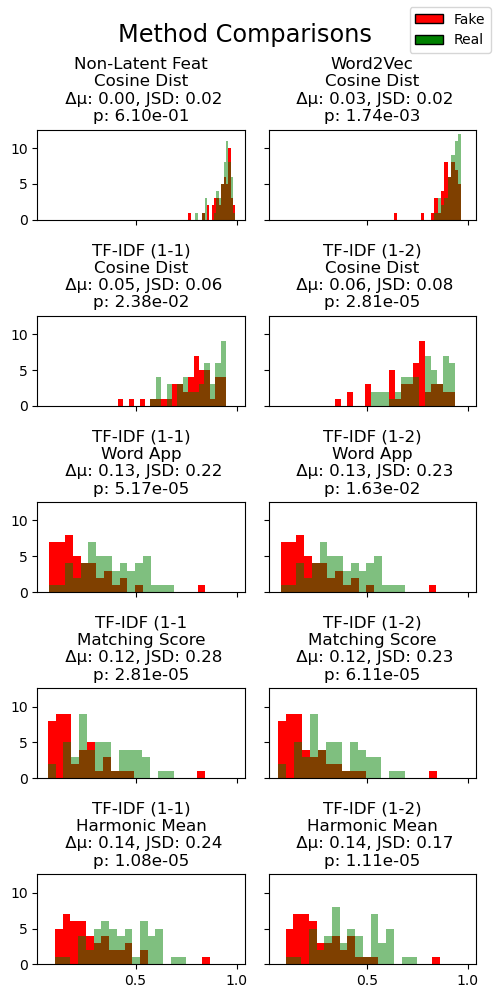
\includegraphics[width=0.5\textwidth]{img/textual_relevance_2.png}
\caption{Textual Relevance}
\label{similarity-metrics}
\end{wrapfigure}
Since we have different similarity metrics, we ought to compare them and select for the one that helps differentiate the \texttt{REAL} and the \texttt{FAKE} articles the best. We will use three methods to aid our selection: $\delta \mu$, Jensen-Shannon Divergence, and ANOVA.

\textbf{$\delta \mu$}, or the difference between the mean of \texttt{REAL} and \texttt{FAKE} articles is a very naive and simplistic measure to compare how differentiated the two distributions are. This measure does not remedy the behaviour of outliers which might significantly shift the mean of the distributions. It also ignores the variance of the distributions. However, it is still a numerically simple metric which would aid us when the distributions are well-formed.

\tododuke{rewrite this}
\textbf{Jensen-Shannon Divergence} "(JSD) is a symmetric version of the Kullback-Leibler Divergence (KL Divergence) used to compare probability distributions. It quantifies dissimilarity between two distributions P and Q. Calculated as (1/2) * KL(P || M) + (1/2) * KL(Q || M), where KL(P || M) and KL(Q || M) are KL Divergences from P and Q to the average distribution M. JSD ranges from 0 to 1; 0 means identical distributions, and 1 means maximally dissimilar. Valuable in information retrieval, natural language processing, and clustering, JSD aids in analyzing and modeling tasks that involve comparing probability distributions (ChatGPT)"

\tododuke{rewrite this}
\textbf{ANOVA}", which stands for Analysis of Variance, and it is a statistical method used to compare the means of multiple groups to determine if there are significant differences between them. The basic idea behind ANOVA is to decompose the total variance in the data into two components: variance between the group means (due to differences between groups) and variance within the groups (due to individual variability and random error). If the variance between the group means is significantly larger than the variance within the groups, it suggests that there are significant differences among the groups' means. We will be using a specific type of ANOVA called one-way repeated measure ANOVA, where you have one independent categorical variable (in this case our label of \texttt{REAL} and \texttt{FAKE}), and several dependent continous variables (in this case our similarity metrics) 'to test for any statistically significant difference between the means of the dependent variables among the groups defined by the independent variable, to reject the null hypothesis that the group means(\texttt{FAKE} and \texttt{REAL}) are equal'.

\subsubsection{Results: similarity metrics}
\tododuke{I can shorten this section if necessary}
We will now discuss our similarity metrics comparison result on table \ref{similarity-metrics}. A good metric should have the fake (in red) and the real (in green) distributions be somewhat well separated. The brown area indicates the overlapping region. Non-latent Cosine Distance is the worst metric with $0 \delta \mu$, $0.02 JSD$, and $6.10e-01 p$, where the two \texttt{FAKE} and \texttt{REAL} distributions are overlapping each other almost at the same point. Word2vec Cosine Distance and TF-IDF(1-1) also perform quite poorly with $\delta \mu$ of 0.03 and 0.05, JSD of 0.02 and 0.06, and p-value of 1.74e-03 and 2.38e-02 respectively. Both these plots have the \texttt{REAL} distribution shifted further to the right but the distributions still overlap significantly, unlike the Non-Laten Cosine Distance, however, these metrics fall below the typical significance level $\alpha$ of 0.05. Although TF-IDF (1-2) Cosine Distance has a similar $\delta \mu$ and JSD of 0.06 and 0.08 respectively, its p-value is markedly low at 2.81e-05. Word App follows a similar pattern where TF-IDF (1-1) and (1-2) produce distinctly different results of 5.17e-05 and 1.63e-02 in p-value, but similar $\delta \mu$ of 0.13 and JSD of 0.22 and 0.23 respectively. We can conclude that the ngram-range of TF-IDF definitely contribute to marked differences in the metrics output. Matching score metrics have similar $\delta \mu$ of 0.12 and JSD range of [0.23, 0.28] with low p-values of 2.81e-05 and 6.11e-05 respectively. The most significant features however are the harmonic mean, combining the previous metrics, with TF-IDF (1-1) at $\delta \mu = 0.14, JSD = 0.24, p = 1.08e-05$ and TF-IDF (1-2) at $\delta \mu = 0.14, JSD = 0.17, p = 1.11e-05$. Since TF-IDF (1-1) yields more difference between the distributions, we will use this as our definitive similarity metric.

% \begin{figure}[H]
%   \centering
%     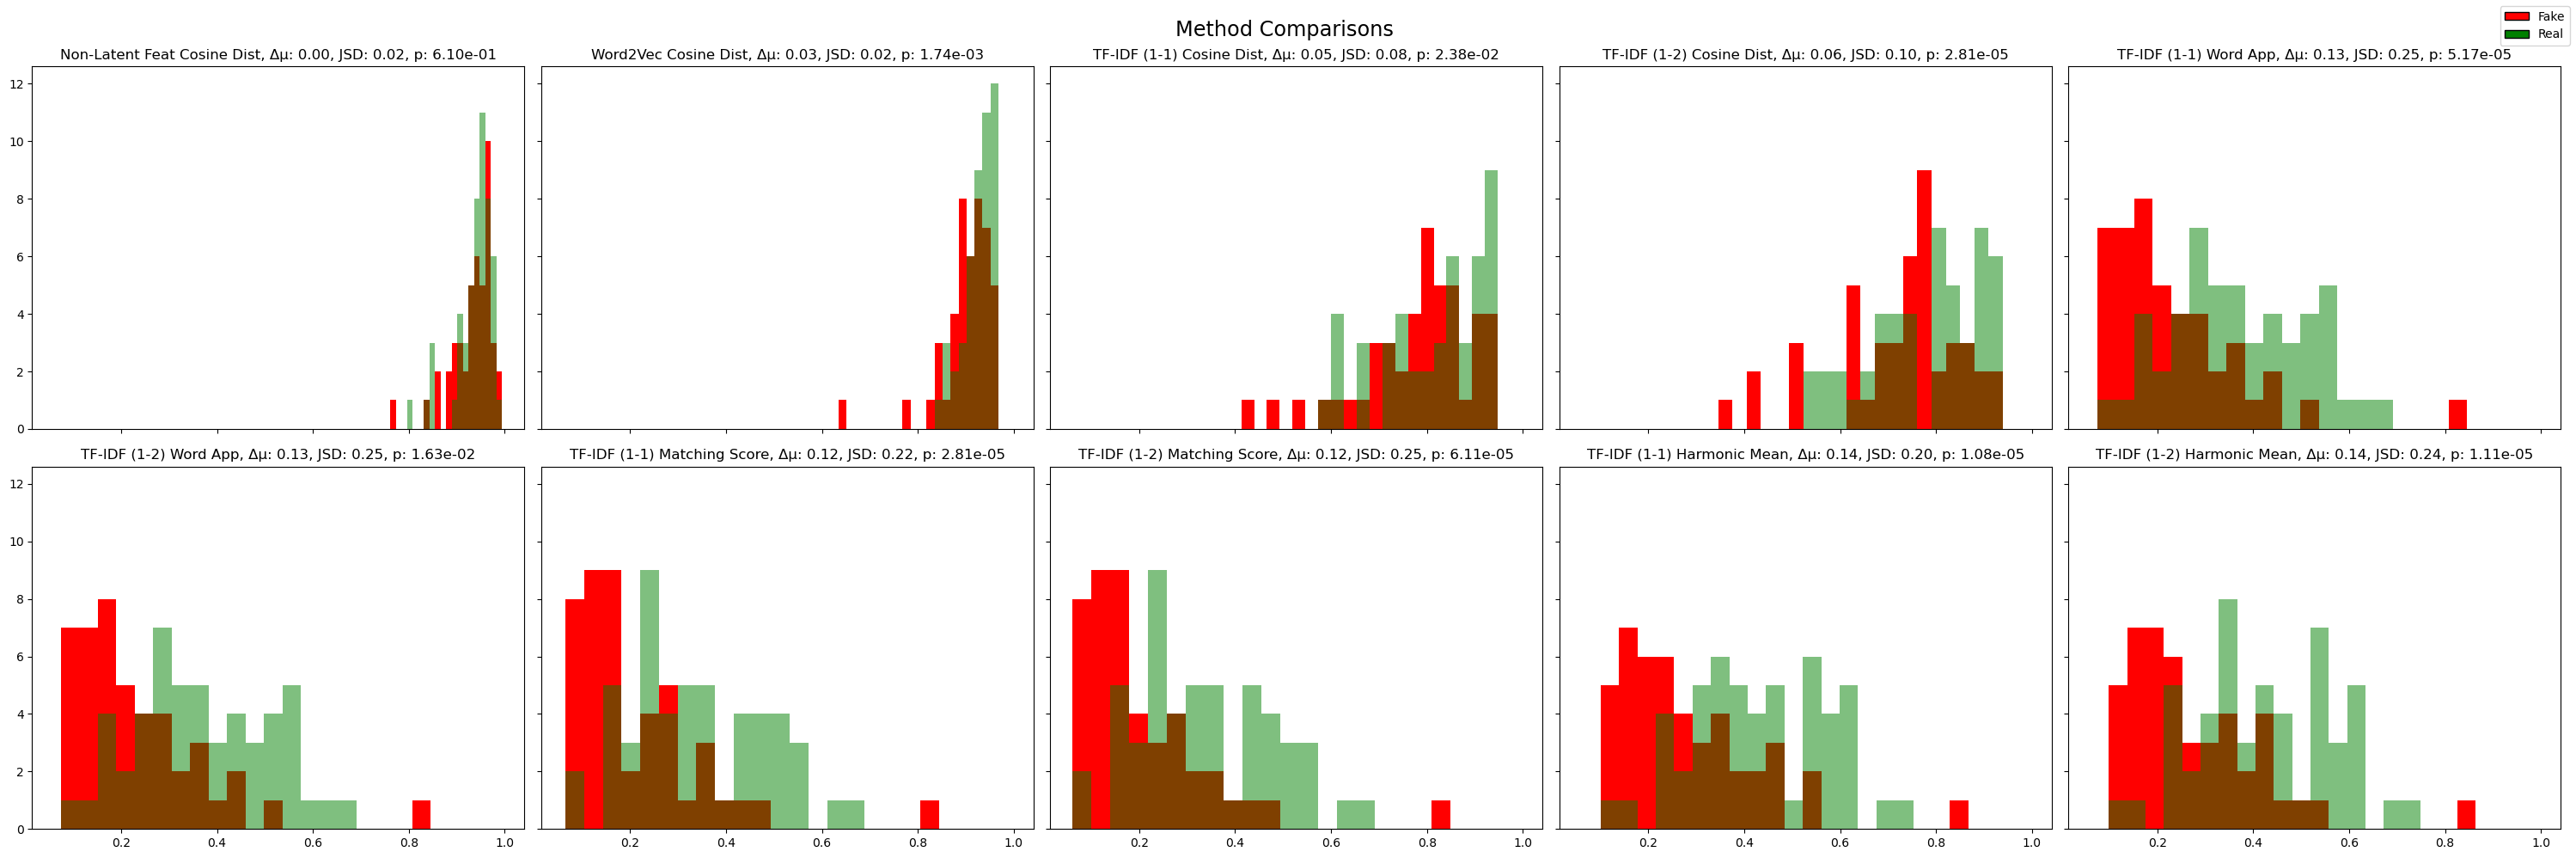
\includegraphics[width=\textwidth]{img/textual_relevance.png}
%     \caption{Textual Relevance}
% \end{figure}

\newsubsection{Normalization and scaling}

\todojim{Write}

\newsubsection{Model --- Machine learning}

\todojim{Write}

\newsubsection{Model --- Neural networks}

\tododhruv{Write}

\newsection{Experimental setup}

\newsubsection{Dataset}

\todojim{write}

\newsubsection{Evaluation metrics}

\todojim{write}

\newsection{Results and discussion}

\todojim{Machine learning}

\tododhruv{Neural nets}

\newsection{Conclusion}

\todoany{Summarise the study and discuss directions for future improvement}

\newsubsection{Limitations}

\todoany{Convert list of limitations to subsubsections with discussion.}

\begin{itemize}
  \item Preprocessing and tokenization was a bit funny:
        \begin{enumerate}
          \item Converting everything to lowercase destroyed acronyms such as ``US''
          \item \verb|nltk| lemmatizer required manually specifying the part of speech to work. We could have used a different library that extracted the POS automatically. Alternatively we could have investigated not lemmatizing at all to maintain proper structure for non-latent features and BERT embeddings.\label{limitation:preprocessing}
        \end{enumerate}
  \item Summary extraction didn't produce perfect results~\label{limitation:summary-extraction}
  \item Article scraping sometimes returned no results even after manually figuring out why~\label{limitation:article-scraping}
  \item Models trained on only US news, may be a problem
\end{itemize}

\cleardoublepage
\pagebreak

\nocite{*}
\printbibliography

\cleardoublepage
\pagebreak

\appendix

\newsection{Individual contributions}

\begin{table}[H]
  \centering
  \begin{tabular}{lll}
    Jim & Dhruv & Duke \\
    \midrule
  \end{tabular}
\end{table}

\subsection{Jim}

\todojim{$\sim$1pg detailing individual contributions}

\subsection{Dhruv}

\tododhruv{$\sim$1pg detailing individual contributions}

\subsection{Duke}

\tododuke{$\sim$1pg detailing individual contributions}

\newsection{Article scraping}\label{appendix:article-scraping}

\begin{table}[H]
  \centering
  \begin{tabular}{cp{8cm}p{3cm}}
    \toprule
    ID & Article extract & Summary\\
    \midrule
    \verb|128_Real| & \small{\articlecontent{128real}} & god wa one never every king november still heart\\
    \midrule
    \verb|2_Fake| & \small{\articlecontent{2fake}} & ha adenugame africanamericans south femi united states africa president donald\\
    \midrule
    \verb|10_Fake| & \small{\articlecontent{10fake}} &wa room hotel maria told employee gonzalez hit video get\\
    \midrule
    \verb|34_Fake| & \small{\articlecontent{34fake}} &trump rage album machine band ha donald music outside year\\
    \bottomrule
  \end{tabular}
  \caption{Articles we were not able to find context articles for.}
\end{table}

\newsection{Non-latent Feature Pearson Correlation Matrix}\label{appendix:correlation-matrx}
\begin{figure}[H]
  \centering
  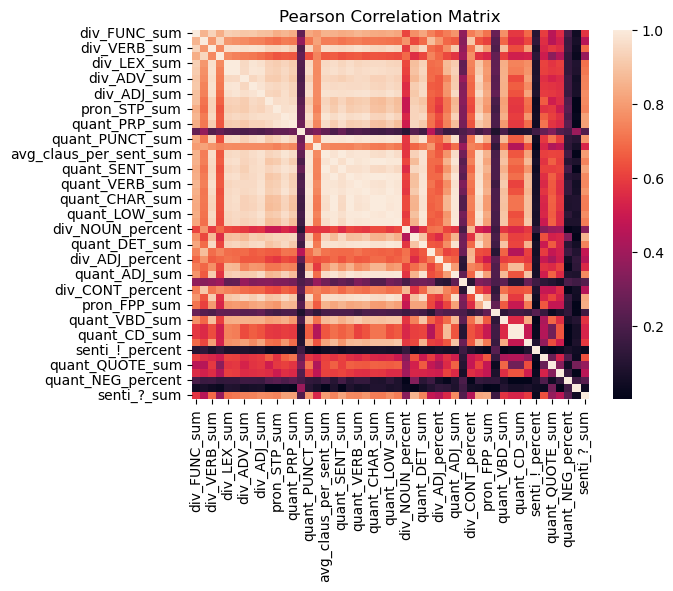
\includegraphics[width=0.8\textwidth]{img/non_latent_corr_matrx.png}
  \caption{Non-Latent Correlation Matrix}
\end{figure}

\end{document}
